% Proseminar
% Sebastian Honegger
% FS15

\documentclass[9pt]{beamer}
\usetheme{Boadilla}  
\usepackage{wrapfig}				% Text umgibt Grafik


\title{Project Sihlstrasse}
%\subtitle{}
\institute[ETH Zurich] {Modelling and Simulating Social Systems\\ETH Zurich}

\author[Filip Meier and Sebastian Honegger]{Filip Meier and Sebastian Honegger}
\date{December 14, 2015}



\begin{document}
\maketitle

\begin{frame}
\frametitle{Overview}
\begin{enumerate}
\item	Introduction project Sihlstrasse
\newline
\item	Project Questions
\newline
\item	Simulation-model
\newline
\item	Implementation of the model
\newline
\item	Assumptions: Unknown parameters
\newline
\item	Results
\newline
\item	Bottleneck?
\newline
\item Conclusion
\end{enumerate}


\end{frame}

\begin{frame}
\frametitle{Introduction project Sihlstrasse}

\begin{figure}[h]
	\centering
		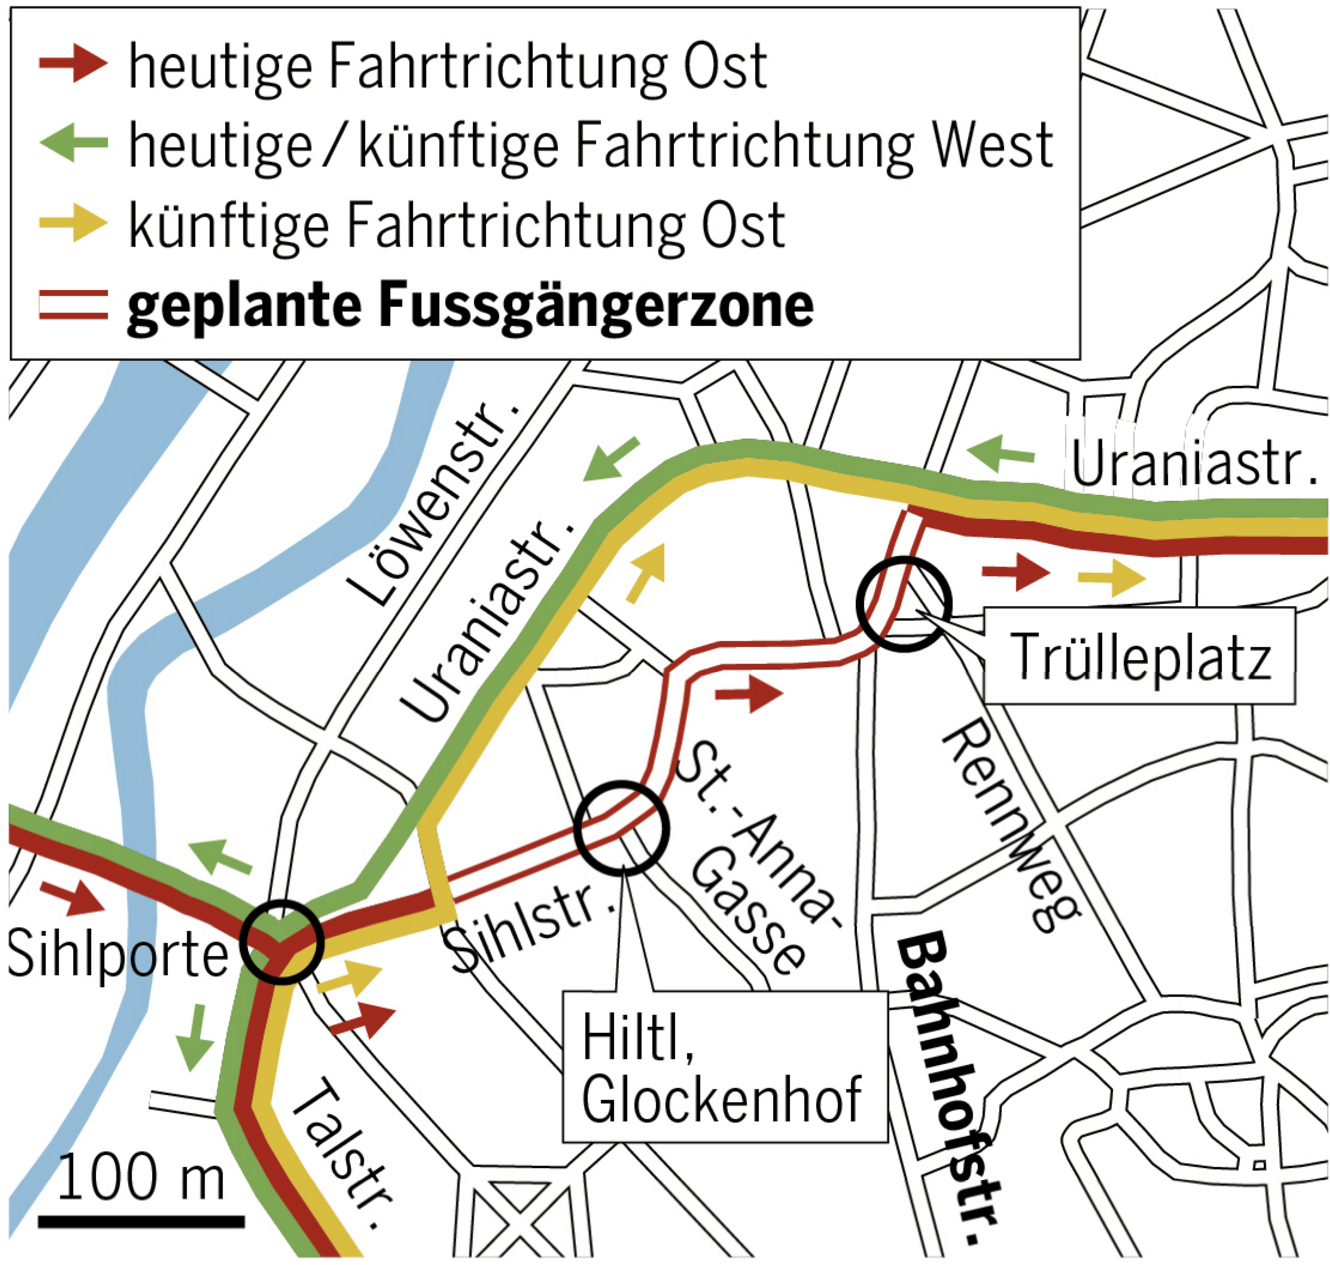
\includegraphics[width=0.6\columnwidth]{Plan_Sihlstrasse.png}
	\caption{\textit{Reference:} Neue Verkehrsorganisation Uraniastrasse (project booklet),\emph{Tiefbauamt Stadt Zuerich,}}
\end{figure}
\end{frame}

\begin{frame}

\frametitle{Project Questions}

\begin{itemize}
\item[1.] Are the streets still large enough to manage the traffic jam peaks on working days?
\item[2.] What is the impact on the neigbourhood streets?
\end{itemize}
\end{frame}


\begin{frame}
\frametitle{Simulation-model}

\textbf{Chowdhury-Schadschneider-model:}\\
\textbf{Start configuration:}\\
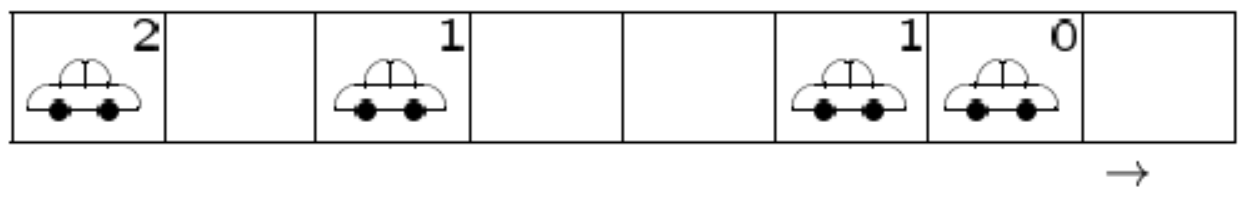
\includegraphics[width=0.7\columnwidth]{config_1.png}
\begin{itemize}
\item[1.] \textbf{Acceleration:}
If $v_n<v_{\mathrm{max}}$ at time $t$, the car $n$ will accelerate is velocity about one unit:
\begin{equation}
v_n \rightarrow v'_n = \min(v_n+1,v_\mathrm{max})
\label{accel_t}
\end{equation}
$v'_n$ represents the new velocity at time $t+1$.
\\
\end{itemize}
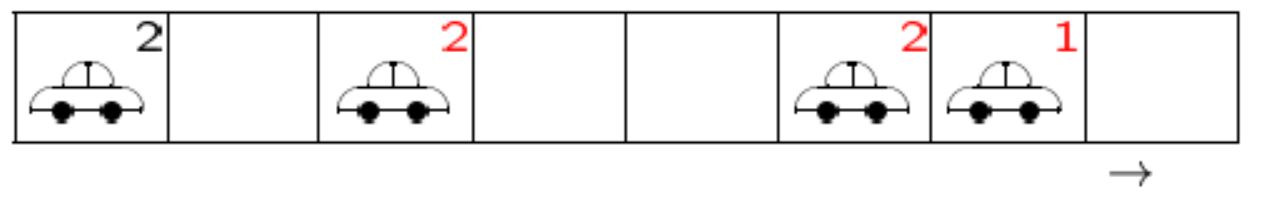
\includegraphics[width=0.7\columnwidth]{config_2.png}\\
\textit{Figure Reference:} Physik des Strassenverkehrs, \emph{Andreas Schadschneider,}http://www.thp.uni-koeln.de
\end{frame}

\begin{frame}
\frametitle{Simulation-model}
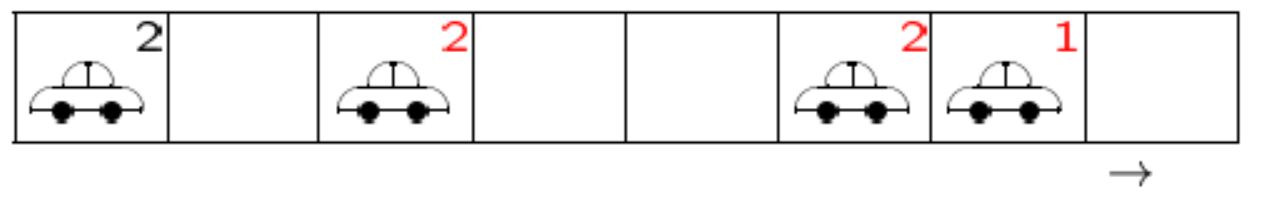
\includegraphics[width=0.7\columnwidth]{config_2.png}
\begin{itemize}
\item[2.]\textbf{Slow down because of cars or traffic lights}
\begin{itemize}
\item[1.]case: The traffic light is red:
\begin{equation}
v'_n \rightarrow \min(v_n,d_n,s_n)
\end{equation}
\item[2.]case: The traffic light is green:
\begin{itemize}
\item[a.] The traffic light get red in the next time step:
\begin{equation}
v'_n \rightarrow \min(v_n,d_n,s_n)
\label{min_lights}
\end{equation}
\item[b.] The traffic light is not getting red:
\begin{equation}
v'_n \rightarrow \min(v_n,d_n)
\end{equation}
\end{itemize}

\end{itemize}
\end{itemize}
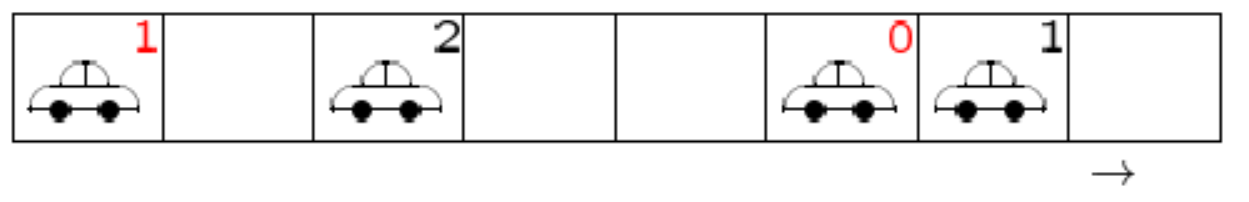
\includegraphics[width=0.7\columnwidth]{config_3.png}\\
\textit{Figure Reference:} Physik des Strassenverkehrs, \emph{Andreas Schadschneider,}http://www.thp.uni-koeln.de
\end{frame}

\begin{frame}
\frametitle{Simulation-model}

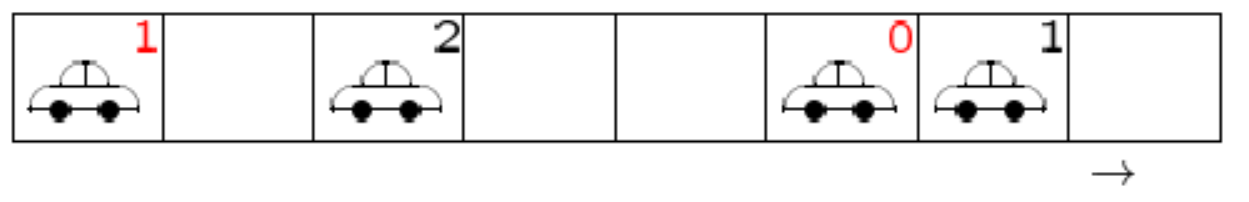
\includegraphics[width=0.7\columnwidth]{config_3.png}
\begin{itemize}
\item[3.]  \textbf{Randomization}
If $v''_n>0$, the velocity of car $n$ will be randomly with the probability $p$ reduced about one unit:
\begin{equation}
v''_n \rightarrow v'''_n=
\begin{cases}
\max(v''_n-1,0) & \mathrm{with\,probability} \quad p\\
v''_n & \mathrm{with\,probability} \quad 1-p
\end{cases}
\label{hangb}
\end{equation}
\end{itemize}
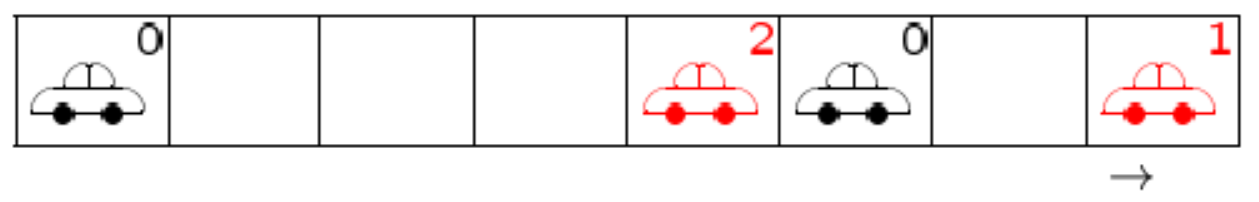
\includegraphics[width=0.7\columnwidth]{config_4.png}\\
\textit{Figure Reference:} Physik des Strassenverkehrs, \emph{Andreas Schadschneider,}http://www.thp.uni-koeln.de
\end{frame}
\begin{frame}
\frametitle{Simulation-model}

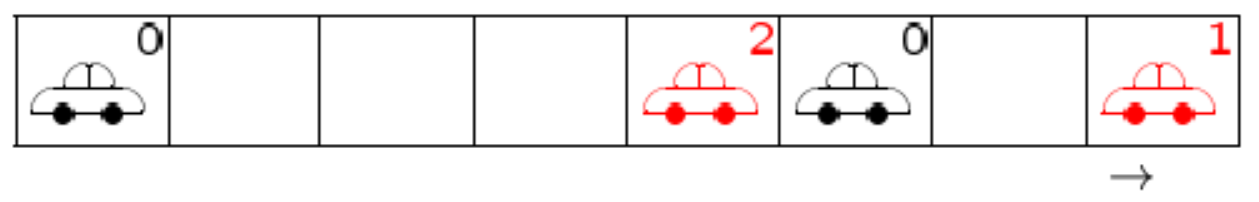
\includegraphics[width=0.7\columnwidth]{config_4.png}
\begin{itemize}
\item[4.] \textbf{Drive:}
The car $n$ drives with the new velocity $v_n(t+1)=v'''_n$ about $v_n(t+1)$ cells:
\begin{equation}
x_n(t+1)=x_n(t)+v_n(t+1)
\label{drive}
\end{equation}
\end{itemize}
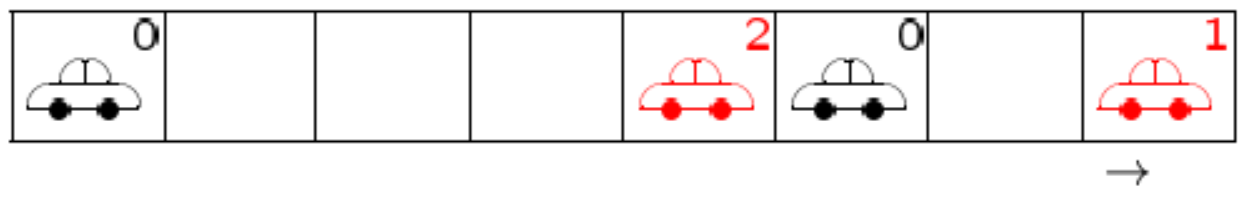
\includegraphics[width=0.7\columnwidth]{config_5.png}

\textit{Figure Reference:} Physik des Strassenverkehrs, \emph{Andreas Schadschneider,}http://www.thp.uni-koeln.de
\label{example_ns} 

\end{frame}

\begin{frame}
\frametitle{Implementation of the model}
\textbf{Color-code for street and velocity:}\\


\vspace{1cm}
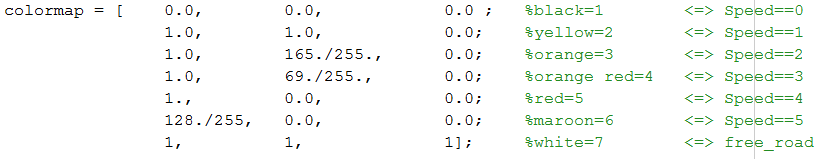
\includegraphics[width=1.\columnwidth]{colormap.png}\vspace{1cm}
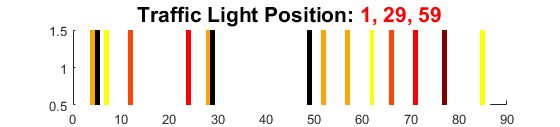
\includegraphics[width=0.75\columnwidth]{tl.png}

\end{frame}

\begin{frame}
\frametitle{Assumptions: Unknown parameters}
\begin{itemize}
\item \textbf{Input:} cars per hour
\begin{itemize}
\item official data set from city of zurich (number of cars which pass traffic light Bahnhofstrasse)
\item values Sihlstrasse:
$[115,74,52,46,51,128,508,719,698,656,691,706,$\\
$607,652,704,732,746,751,729,559,397,335,325,247]$
\end{itemize}
\vspace{.5cm}
\item \textbf{Traffic lights:} 
\begin{itemize}
\item Position: -
\item 4 steps red, 11 steps green (synchronous: green $\Leftrightarrow$ red)
\end{itemize}
\vspace{0.5cm}
\item \textbf{Output:} cars per hour
\begin{itemize}
\item last traffic light... 

\item Output: 600 cars/hour

\end{itemize}

\end{itemize}

\end{frame}

\begin{frame}
\frametitle{Results}

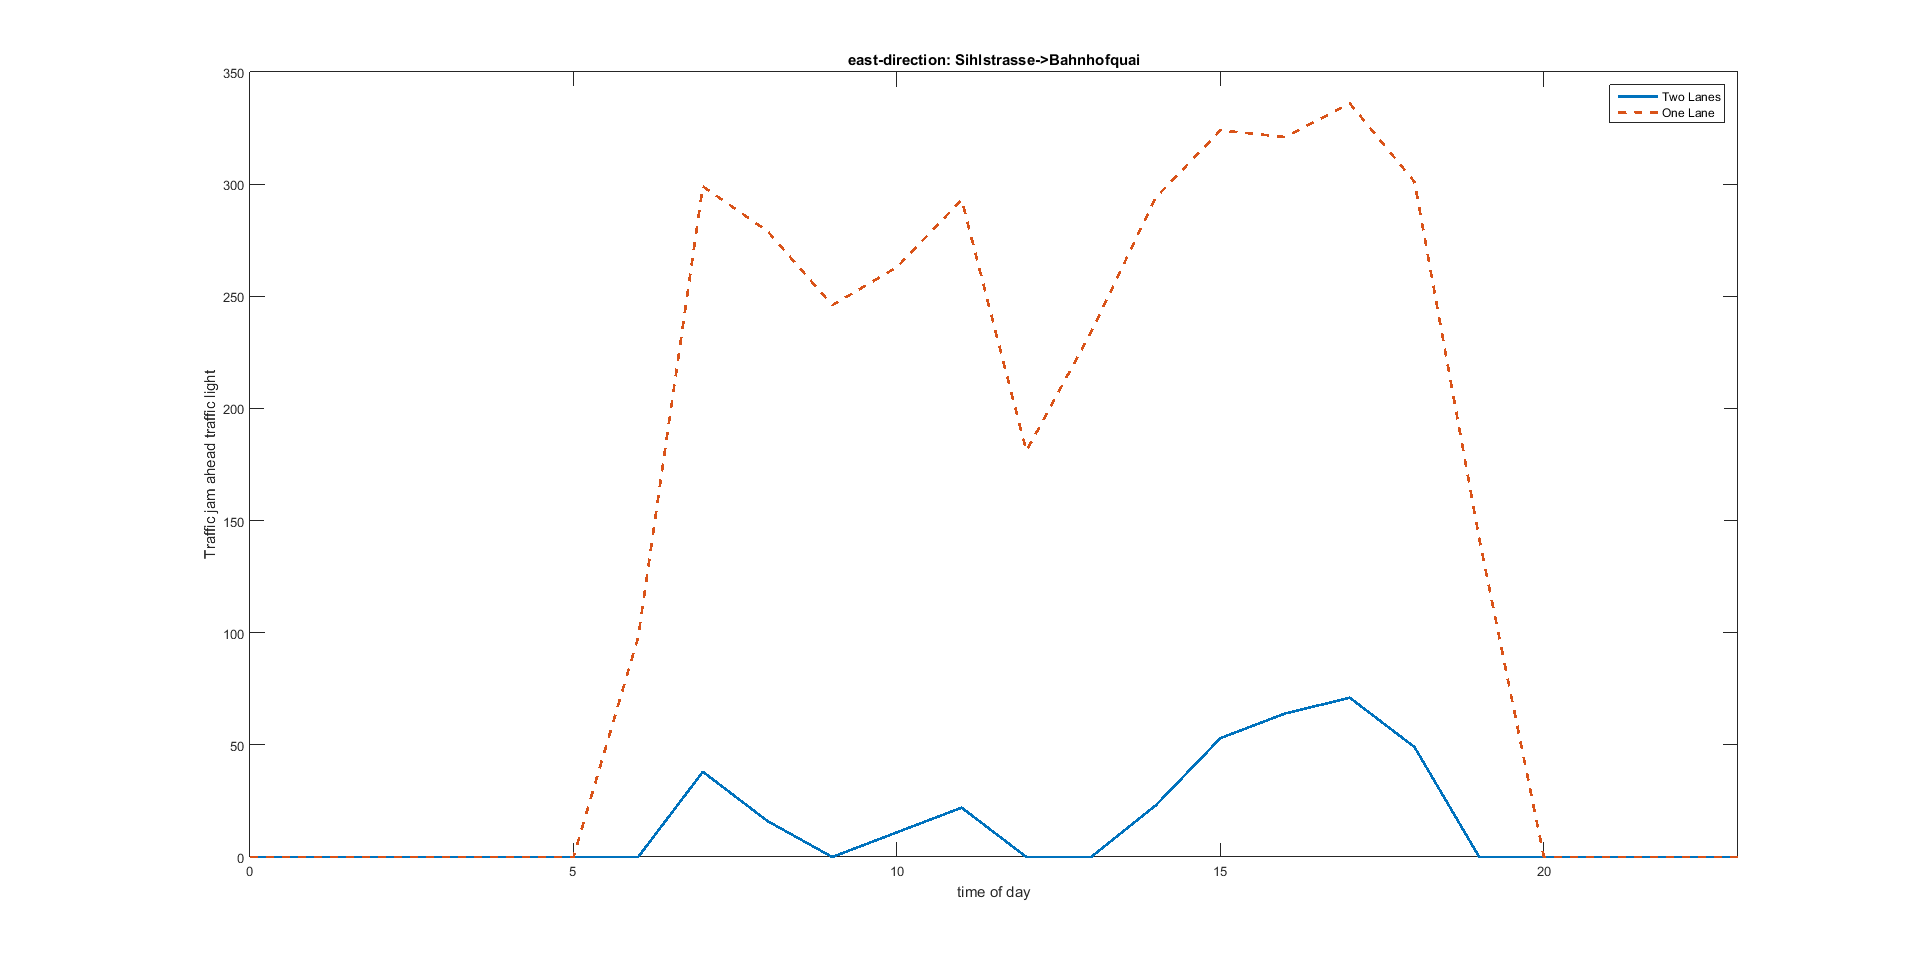
\includegraphics[width=1.\columnwidth]{Comparison_Traffic_jam.png}
\begin{itemize}
\item \textbf{Traffic jam:} around 300 cars ($\approx 2.2\,\mathrm{km}$) more at the peak times
\item Reasons:
\begin{itemize}
\item less space for cars (one lane): $+86$ cars
\item less throughput of the street: $+200$ cars
\end{itemize}
\end{itemize}
\end{frame}

\begin{frame}
\frametitle{Bottleneck?}
\begin{itemize}
\item \textit{"Diese Verkehrsmenge auf der Ausweichroute kann zu den Hauptverkehrszeiten weder zusaetzlich am Knoten Sihlporte noch am Knoten Urania-/Bahnhofstrasse verarbeitet werden. Dies hat aber keinen Einfluss auf die tatsaechliche Kapazitaet, weil ohnehin der Knoten Uraniastrasse/Bahnhofquai leistungsbestimmend ist, sowohl heute wie im zukünftigen Zustand."} (City of Zurich, project booklet)
\end{itemize}

\begin{figure}[H]
\begin{minipage}[t]{.5\textwidth}
\begin{itemize}
\item What if:
\begin{itemize}
\item Traffic lights: always green
\item Output: $\infty$
\end{itemize}
\vspace{1cm}
\item Conclusion:
\begin{itemize}
\item bottleneck is not given by the last traffic light (Output) \textbf{if} the capacity is bigger than 600 cars per hour.

\end{itemize}
\end{itemize}

\end{minipage}\hfill
\begin{minipage}[t]{.5\textwidth}
	\centering
	\vspace{0pt}
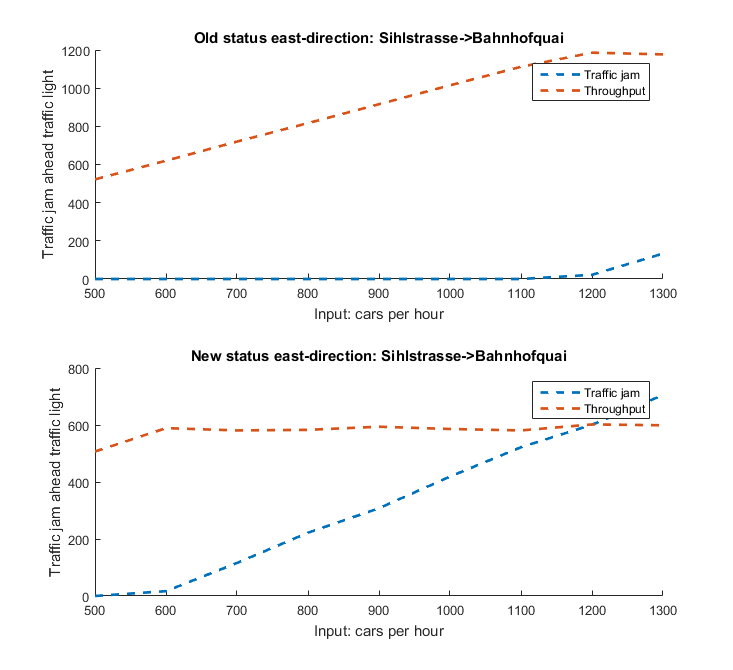
\includegraphics[width=\textwidth]{max_throughput2.png}
\end{minipage}\hfill
\end{figure}

\end{frame}

\begin{frame}
\frametitle{Conclusion}

\begin{itemize}
\item Simulation is working for both situations: 
\begin{itemize}
\item one  lane or two lanes
\item both direction
\item different parameters (input, output)
\end{itemize}
\vspace{1cm}
\item 300 cars more for the one lane simulation, high impact on the neighbourhood streets
\vspace{1cm}
\item Future improvements:
\begin{itemize}
\item traffic light set-up: red and green circuit (asynchronous)  
\end{itemize}

\end{itemize}

\end{frame}

\end{document}





